\documentclass{river-journal}
\usepackage{rivps}
\usepackage[mtbold]{mathtime}

\usepackage{graphicx}
\usepackage{graphics}
\usepackage{subfigure}
\usepackage{cite}

% for alternatives, see appendix of manual

\newtheorem{guess}{Conjecture}

% bibliographies
\bibliographystyle{plain}
% also tested with natbib

\raggedbottom
\sloppy\par

\begin{document}
\begin{opening}
\title{A Sample Document}
\author{Leslie Lamport}
\institute{Author's Affiliation,  \texttt{no@spam}}
\end{opening}

\runningtitle{Sample Document}
\runningauthor{L. Lamport}

\subsection*{Abstract}
This is a sample input file.  Comparing it with the output it
generates can show you how to produce a simple document of
your own.

\keywords{sample, \LaTeX}

\section{Normal Text}

The ends  of words and sentences are marked
  by   spaces. It  doesn't matter how many
spaces    you type; one is as good as 100.  The
end of   a line counts as a space.

One   or more   blank lines denote the  end
of  a paragraph.

Since any number of consecutive spaces are treated like a single
one, the formatting of the input file makes no difference to
      \TeX,         % The \TeX command generates the TeX logo.
but it makes a difference to you.
When you use
      \LaTeX,       % The \LaTeX command generates the LaTeX logo.
making your input file as easy to read as possible
will be a great help as you write your document and when you
change it.  This sample file shows how you can add comments to
your own input file.

Because printing is different from typewriting, there are a
number of things that you have to do differently when preparing
an input file than if you were just typing the document directly.
Quotation marks like
       ``this''
have to be handled specially, as do quotes within quotes:
       ``\,`this'                  % \, separates the double and single quote.
    is what I just
    wrote, not  `that'\,''.

Dashes come in three sizes: an
       intra-word
dash, a medium dash for number ranges like
       1--2,
and a punctuation
       dash---like
this.

A sentence-ending space should be larger than the space between words
within a sentence.  You sometimes have to type special commands in
conjunction with punctuation characters to get this right, as in the
following sentence.
       Gnats, gnus, etc.\    % `\ ' makes an inter-word space.
       all begin with G\@.   % \@ marks end-of-sentence punctuation.
You should check the spaces after periods when reading your output to
make sure you haven't forgotten any special cases.
Generating an ellipsis
       \ldots\    % `\ ' needed because TeX ignores spaces after
          % command names like \ldots made from \ + letters.
          %
          % Note how a `%' character causes TeX to ignore the
          % end of the input line, so these blank lines do not
          % start a new paragraph.
with the right spacing around the periods
requires a special  command.

\TeX\ interprets some common characters as commands, so you must type
special commands to generate them.  These characters include the
following:
       \$ \& \% \# \{ and~\}.

In printing, text is emphasized by using an
       {\em italic\/}  % The \/ command produces the tiny extra space that
               % should be added between a slanted and a following
               % unslanted letter.
type style.

\begin{em}
   A long segment of text can also be emphasized in this way.  Text within
   such a segment given additional emphasis
      with\/ {\em Roman}
   type.  Italic type loses its ability to emphasize and become simply
   distracting when used excessively.
\end{em}

It is sometimes necessary to prevent \TeX\ from breaking a line where
it might otherwise do so.  This may be at a space, as between the
``Mr.'' and ``Jones'' in
       ``Mr.~Jones'',        % ~ produces an unbreakable interword space.
or within a word---especially when the word is a symbol like
       \mbox{\em itemnum\/}
that makes little sense when hyphenated across
       lines.





\TeX\ is good at typesetting mathematical formulas like
       \( x-3y = 7 \)
or
       \( a_{1} > x^{2n} / y^{2n} > x' \).
Remember that a letter like
       $x$        % $ ... $  and  \( ... \)  are equivalent
is a formula when it denotes a mathematical symbol, and should
be treated as one.


\section{Notes}
Footnotes\footnote{This is an example of a footnote.}
pose no problem.\footnote{And another one.}


\section{Displayed Text}

The following is an example of an {\em itemized} list.
\begin{itemize}
\item  This is the first item of an itemized list.  Each item
      in the list is marked with a ``tick''.  The document
      style determines what kind of tick mark is used.
\item  This is the second item of the list.  It contains another
      list nested inside it.  The inner list is an {\em enumerated}
      list.
    \begin{enumerate}
       \item This is the first item of an enumerated list that
            is nested within the itemized list.
          \item This is the second item of the inner list.  \LaTeX\
            allows you to nest lists deeper than you really should.
      \end{enumerate}
      This is the rest of the second item of the outer list.  It
      is no more interesting than any other part of the item.
   \item  This is the third item of the list.
\end{itemize}


The following is an example of an {\em enumerated} list, two levels deep.
\begin{enumerate}
\item  This is the first item of an enumerated list.  Each item
      in the list is marked with a letter or number.  The document
      style determines what kind of mark is used.
\item  This is the second item of the list.  It contains another
      enumerated list nested inside it.
    \begin{enumerate}
       \item This is the first item of an enumerated list that
            is nested within the enumerated list.
          \item This is the second item of the inner list.  \LaTeX\
            allows you to nest lists deeper than you really should.
      \end{enumerate}
      This is the rest of the second item of the outer list.  It
      is no more interesting than any other part of the item.
   \item  This is the third item of the list.
\end{enumerate}


The following is an example of a {\em description} list.
\begin{description}
\item[Cow] Highly intelligent animal that can produce milk out of grass.
\item[Horse] Less intelligent animal renowned for its legs.
\item[Human being] Not so intelligent animal that thinks that it can think.
\end{description}

Quotations are implemented as lists. Here comes a sample quotation,
repeated once to test paragraph indentation of additional
paragraphs.
\begin{quotation}
Quotations are implemented as lists. Here comes a sample quotation,
repeated once to test paragraph indentation of additional paragraphs.

Quotations are implemented as lists. Here comes a sample quotation,
repeated once to test paragraph indentation of additional paragraphs.
\end{quotation}

Mathematical formulas may also be displayed.  A displayed formula is
one-line long; multiline formulas require special formatting
instructions.
   \[  x' + y^{2} = z_{i}^{2}\]
Don't start a paragraph with a displayed equation, nor make
one a paragraph by itself.

Example of a theorem:


\begin{guess}
All conjectures are interesting, but some conjectures are more
interesting than others.
\end{guess}


\section{Tables and Figures}

Cross reference should be labelled, e.g., as you can see in
Table~\ref{sphericcase} and also in Table~\ref{parset}.


\begin{table} %
\caption[]{Parameter set used in the model of Bunt \cite{Bunt}. }\label{parset}
\begin{tabular}{lrl}
\hline
$Q_{s,\max}$   & [g/g DM h]  & 0.18\\
$K_{s}$       & [g/L]        & 1.0\\
$Y_{x/s}$     & [g DM/g]     & 0.5\\
$Y_{p/s}$     & [g/g]        & 0.854\\
$Q_{p,\max}$   & [g/g DM h]  & 0.0045\\
$\mu_{\rm crit}$  & [h$^{-1}$]  & 0.01\\
$k_{h}$       & [h$^{-1}$]  & 0.002\\
$m_{s}$       & [g/g DM h]  & 0.025\\
\hline
\end{tabular}
\end{table}

\begin{table*}
\caption[]{The spherical case ($I_1=0$, $I_2=0$).}
\label{sphericcase}
\begin{tabular}{crrrrc}
\hline
Equil. \\
Points & \multicolumn{1}{c}{$x$} & \multicolumn{1}{c}{$y$} & \multicolumn{1}{c}{$z$} & \multicolumn{1}{c}{$C$} &
S \\
\hline
$~~L_1$ & $-$2.485252241 & 0.000000000 & 0.017100631 & 8.230711648 & U \\
$~~L_2$ &    0.000000000 & 0.000000000 & 3.068883732 & 0.000000000 & S \\
$~~L_3$ &    0.009869059 & 0.000000000 & 4.756386544 & $-$0.000057922 & U \\
$~~L_4$ &    0.210589855 & 0.000000000 & $-$0.007021459 & 9.440510897 & U \\
$~~L_5$ &    0.455926604 & 0.000000000 & $-$0.212446624 & 7.586126667 & U \\
$~~L_6$ &    0.667031314 & 0.000000000 & 0.529879957 & 3.497660052 & U \\
$~~L_7$ &    2.164386674 & 0.000000000 & $-$0.169308438 & 6.866562449 & U \\
$~~L_8$ &    0.560414471 & 0.421735658 & $-$0.093667445 & 9.241525367 & U \\
$~~L_9$ &    0.560414471 & $-$0.421735658 & $-$0.093667445 & 9.241525367 & U
\\
$~~L_{10}$ & 1.472523232 & 1.393484549 & $-$0.083801333 & 6.733436505 & U \\
$~~L_{11}$ & 1.472523232 & $-$1.393484549 & $-$0.083801333 & 6.733436505 & U
\\ \hline
\end{tabular}
\end{table*}


A major point of difference lies in the value of the specific
production rate $\pi$ for large values of the specific growth rate
$\mu$.  Already in the early publications \cite{Falzon87} it
appeared that high glucose concentrations in the production phase
are well correlated with a low penicillin yield (the `glucose
effect'). It has been confirmed recently
\cite{Bunt,Cahour-thesis,BrownAndBurton,Carr-Goldstein}
that
high glucose concentrations inhibit the synthesis of the enzymes of the
penicillin pathway, but not the actual penicillin biosynthesis.
In other words, glucose represses (and not inhibits) the penicillin
biosynthesis.

These findings do not contradict the results of
\cite{Chin88-book} (on which Bunt \cite{Bunt} based their
production kinetics) and of \cite{ChinThesis} which were
obtained for continuous culture fermentations.  Because for high
values of the specific growth rate $\mu$ it is most likely (as shall
be discussed below) that maintenance metabolism occurs, it can be
shown that in steady state continuous culture conditions, and with
$\mu$ described by a Monod kinetics
\begin{equation}
    C_{s}  =  K_{M} \frac{\mu/\mu_{x}}{1-\mu/\mu_{x}} \label{cs}
\end{equation}
Pirt and Rhigelato determined $\pi$ for $\mu$ between
$0.023$ and $0.086$ h$^{-1}$.
They also reported a value $\mu_{x} \approx 0.095$
h$^{-1}$, so that for their experiments $\mu/\mu_{x}$ is in the range
of $0.24$ to $0.9$.
Substituting $K _M$ in Eq. (\ref{cs}) by
the value $K_{M}=1$ g/L as used by Bunt \cite{Bunt}, one finds
with the above equation $0.3 < C_{s} < 9$ g/L. This agrees well with
the work of Bunt \cite{Bunt}, who reported that penicillin biosynthesis
repression only occurs at glucose concentrations from $C_{s}=10$ g/L on.
The conclusion is that the glucose concentrations in the experiments of
Pirt and Rhigelato probably were too low for glucose repression to be
detected. The experimental data published by Ryu and Hospodka
are not detailed sufficiently to permit a similar analysis.



\begin{table}
\caption[]{Parameter sets used by Bajpai and Reu{\ss}.}
\begin{tabular}{lrll}
\hline
\multicolumn{2}{l}{\it parameter} & {\it Set 1} & {\it Set 2}\\
\hline
$\mu_{x}$           & [h$^{-1}$]  & 0.092       & 0.11          \\
$K_{x}$             & [g/g DM]     & 0.15        & 0.006         \\
$\mu_{p}$           & [g/g DM h]  & 0.005       & 0.004         \\
$K_{p}$             & [g/L]        & 0.0002      & 0.0001        \\
$K_{i}$             & [g/L]        & 0.1         & 0.1           \\
$Y_{x/s}$           & [g DM/g]     & 0.45        & 0.47          \\
$Y_{p/s}$           & [g/g]        & 0.9         & 1.2           \\
$k_{h}$             & [h$^{-1}$]  & 0.04        & 0.01          \\
$m_{s}$             & [g/g DM h]  & 0.014       & 0.029         \\
\hline
\end{tabular}
\end{table}

Bajpai and Reu{\ss} decided to disregard the
differences between time constants for the two regulation mechanisms
(glucose repression or inhibition) because of the
relatively very long fermentation times, and therefore proposed a Haldane
expression for $\pi$.

It is interesting that simulations with the \cite{Bunt} model for the
initial conditions given by these authors indicate that, when the
remaining substrate is fed at a constant rate, a considerable and
unrealistic amount of penicillin is
produced when the glucose concentration is still very high \cite{CarberryCL88}
Simulations with the Bajpai and Reu\ss\ model correctly predict almost
no penicillin production in similar conditions.


The maintenance coefficient used by Bunt \cite{Bunt}
($m_{s}=0.025$ g/g DM h) corresponds well to
the value $m_{s}=0.029$ g/g DM h (Set 2 of \cite{BuchananRBES}), to the
value $m_{s}=0.024$ g/g DM h reported in \cite{MMI2-d3}, and to the
value used in \cite{CawseyIJMMS} ($m_{s}=0.022$ g/g DM h) (1983).
However, these values differ from the value in Set 1 of
\cite{BuchananRBES} ($m_{s}=0.014$ g/g DM h).
It is not clear where this difference originated from.
Simulations indicated that the dynamic behaviour of the model is rather
sensitive with respect to the value of $m_{s}$.

In the model of Bunt \cite{Bunt}, at severe substrate limitation
conditions, and thus most probably corresponding to endogenous
metabolic behaviour, the biomass consumption due to maintenance and
production requirements may exceed the conversion of substrate into
biomass and $\mu$ eventually may become negative. This situation may
occur at the end of the growth phase during a fed-batch
fermentation.  For these conditions $\pi$ is not defined. A
straightforward extension of the $\pi(\mu)$ kinetics (10) could be
$\pi(\mu \leq 0)=0$, but there are some biochemical indications that
the penicillin biosynthesis actually does not stop in that case.

\begin{figure}
\centerline{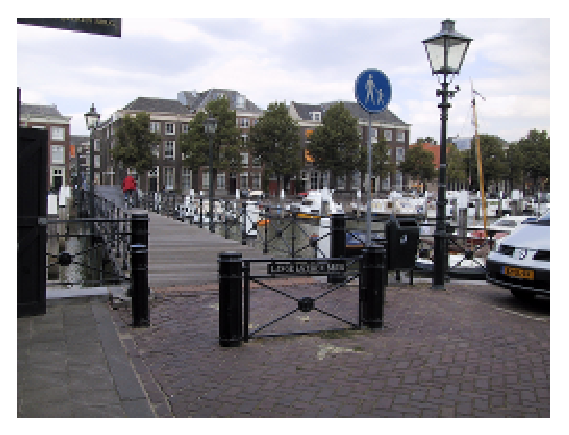
\includegraphics[width=3in]{bridge}}
\caption[]{Lange ijzeren brug, Dordrecht, The Netherlands.}%
\label{bridge}
\end{figure}

Sample of cross-reference to a figure:
Figure~\ref{bridge} shows a color image.

\section{Headings}

\subsection{Subsection}
\cite{Carr-Goldstein,Cohen-Jones88-book}
based their model on balancing methods and biochemical
knowledge. The original model (1980) contained an equation for the
oxygen dynamics which has been omitted in a second paper
(1981). This simplified model shall be discussed here.

\subsubsection{Subsubsection}
Carr and Goldstein \cite{Carr-Goldstein}
based their model on balancing methods and biochemical
knowledge. The original model (1980) contained an equation for the
oxygen dynamics which has been omitted in a second paper
(1981). This simplified model shall be discussed here.

\paragraph{Paragraph.}
Carr and Goldstein \cite{Carr-Goldstein}
based their model on balancing methods and biochemical
knowledge. The original model (1980) contained an equation for the
oxygen dynamics which has been omitted in a second paper
(1981). This simplified model shall be discussed here.

\section{Equations and the Like}

Two equations:
\begin{equation}
    C_{s}  =  K_{M} \frac{\mu/\mu_{x}}{1-\mu/\mu_{x}} \label{ccs}
\end{equation}
and
\begin{equation}
    G = \frac{P_{\rm opt} - P_{\rm ref}}{P_{\rm ref}} \mbox{\ }100 \mbox{\ }(\%)
\end{equation}

Two equation arrays:
\begin{eqnarray}
  \frac{dS}{dt} & = & - \sigma X + s_{F} F\\
  \frac{dX}{dt} & = &   \mu    X\\
  \frac{dP}{dt} & = &   \pi    X - k_{h} P\\
  \frac{dV}{dt} & = &   F
\end{eqnarray}
and
\begin{eqnarray}
 \mu_{\rm substr} & = & \mu_{x} \frac{C_{s}}{K_{x}C_{x}+C_{s}}  \\
 \mu              & = & \mu_{\rm substr} - Y_{x/s}(1-H(C_{s}))(m_{s}+\pi /Y_{p/s}) \\
 \sigma           & = & \mu_{\rm substr}/Y_{x/s}+ H(C_{s}) (m_{s}+ \pi /Y_{p/s})
\end{eqnarray}

Let us also recall the very first equation \ref{cs}.

\appendix

And this is my Appendix.

\subsection*{Appendix Subsection}

Some text.

\nocite{*} % add all entries from sample.bib

%\bibliography{sample}
\begin{thebibliography}{10}

\bibitem{BrownAndBurton}
J.S. Brown and R.R. Burton.
Diagnostic models for procedural bugs in basic mathematical skills.
{\em Cognitive Science}, 2(2):155--192, 1978.

\bibitem{BuchananRBES}
B.G. Buchanan and E.H. Shortliffe.
{\em Rule-Based Expert Systems: The MYCIN Experiments of the Stanford
  Heuristic Programming Project}.
Addison-Wesley Publishing Company, 1984.

\bibitem{Bunt}
H.C. Bunt.
 Modular incremental modelling of belief and intention.
 In {\em Proceedings of the Second International Workshop on User
  Modeling}, 1990.

\bibitem{Cahour-90-Montreal}
B. Cahour.
 Competence modelling in consultation dialogs.
 In L. Berlinguet and D. Berthelette (Eds.), {\em Proceedings
  of the International Congress, Work with Dispay Units 89}, North Holland, Amsterdam, 1990. 

\bibitem{Cahour-thesis}
B. Cahour.
 {La mod{\'e}lisation de l'interlocuteur: Elaboration du
  mod{\`e}le et effets au cours de dialogues de consultation}.
 PhD Thesis, Universit{\'e} Paris, France, 1991.

\bibitem{CarberryCL88}
S.M. Carberry.
 Modeling the user's plans and goals.
 {\em Computational Linguistics}, 14(3):23--37, 1988.

\bibitem{CarbonellScholar}
J.R. Carbonell.
 AI in CAI: An artificial intelligence approach to computer-aided
  instruction.
 {\em IEEE Transactions on Man-Machine Systems}, 11:190--202, 1970.

\bibitem{Carr-Goldstein}
B. Carr and I. Goldstein.
 Overlays: A theory of modelling for computed aided instruction.
 AI Memo 406, 1977.

\bibitem{CawseyIJMMS}
A. Cawsey.
 Planning interactive explanations.
 {\em International Journal of Man-Machine Studies}, in press.

\bibitem{chandra-swartout}
B. Chandrasekaran and W. Swartout.
 Explanations in knowledge systems: The role of explicit
  representation of design knowledge.
 {\em IEEE Expert}, 6(3):47--50, 1991.

\bibitem{MMI2-d3}
H. Chappel and B. Cahour.
 User modeling for multi-modal co-operative dialogue with KBS.
 Deliverable D3, Esprit Project P2474, 1991.

\bibitem{ChinThesis}
D.N. Chin.
 {Intelligent agents as a basis for natural language interfaces}.
 PhD Thesis, University of California at Berkeley, 1987.

\bibitem{Chin88-book}
D.N. Chin.
 {KNOME}: {M}odeling what the user knows in {UC}.
 In A. Kobsa and W. Wahlster (Eds.), {\em User Models in
  Dialog Systems}. Springer-Verlag, Berlin, 1989.

\bibitem{Cohen-Jones88-book}
R. Cohen and M. Jones.
 Incorporating user models into expert systems for educational
  diagnosis.
 In A. Kobsa and W. Wahlster (Eds.), {\em User Models in
  Dialog Systems}, pp.~35--51. Springer-Verlag,   Berlin, 1989.

\bibitem{Falzon87}
P. Falzon.
 Les dialogues de diagnostic: L'{\'e}valuation des connaissances de
  l'interlocuteur.
 Technical Report 747, INRIA, Rocquencourt, France, 1987.

\bibitem{FininJoshiWebber}
T.W. Finin, A.K. Joshi, and B.L. Webber.
 Natural language interactions with artificial experts.
 {\em Proceedings of the IEEE}, 74(7), 1986.

\end{thebibliography}

\section*{Biography}

\fbox{\parbox[t]{3cm}{Here is space for \\
a photograph of \\
the author. \\
\vspace*{2cm}
}}

\medskip
\noindent
{\bf Author's name}. A short vitae can be included here.

\end{document}
